\documentclass[journal]{vgtc}                % final (journal style)
%\documentclass[review,journal]{vgtc}         % review (journal style)
%\documentclass[widereview]{vgtc}             % wide-spaced review
%\documentclass[preprint,journal]{vgtc}       % preprint (journal style)

%% Uncomment one of the lines above depending on where your paper is
%% in the conference process. ``review'' and ``widereview'' are for review
%% submission, ``preprint'' is for pre-publication, and the final version
%% doesn't use a specific qualifier.

%% Please use one of the ``review'' options in combination with the
%% assigned online id (see below) ONLY if your paper uses a double blind
%% review process. Some conferences, like IEEE Vis and InfoVis, have NOT
%% in the past.

%% Please note that the use of figures other than the optional teaser is not permitted on the first page
%% of the journal version.  Figures should begin on the second page and be
%% in CMYK or Grey scale format, otherwise, colour shifting may occur
%% during the printing process.  Papers submitted with figures other than the optional teaser on the
%% first page will be refused. Also, the teaser figure should only have the
%% width of the abstract as the template enforces it.

%% These few lines make a distinction between latex and pdflatex calls and they
%% bring in essential packages for graphics and font handling.
%% Note that due to the \DeclareGraphicsExtensions{} call it is no longer necessary
%% to provide the the path and extension of a graphics file:
%% 
\includegraphics{diamondrule} is completely sufficient.
%%
\ifpdf%                                % if we use pdflatex
  \pdfoutput=1\relax                   % create PDFs from pdfLaTeX
  \pdfcompresslevel=9                  % PDF Compression
  \pdfoptionpdfminorversion=7          % create PDF 1.7
  \ExecuteOptions{pdftex}
  \usepackage{graphicx}                % allow us to embed graphics files
  \DeclareGraphicsExtensions{.pdf,.png,.jpg,.jpeg} % for pdflatex we expect .pdf, .png, or .jpg files
\else%                                 % else we use pure latex
  \ExecuteOptions{dvips}
  \usepackage{graphicx}                % allow us to embed graphics files
  \DeclareGraphicsExtensions{.eps}     % for pure latex we expect eps files
\fi%

%% it is recomended to use ``\autoref{sec:bla}'' instead of ``Fig.~\ref{sec:bla}''
\graphicspath{{figures/}{pictures/}{images/}{./}} % where to search for the images

\usepackage{microtype}                 % use micro-typography (slightly more compact, better to read)
\PassOptionsToPackage{warn}{textcomp}  % to address font issues with \textrightarrow
\usepackage{textcomp}                  % use better special symbols
\usepackage{mathptmx}                  % use matching math font
\usepackage{times}                     % we use Times as the main font
\renewcommand*\ttdefault{txtt}         % a nicer typewriter font
\usepackage{cite}                      % needed to automatically sort the references
\usepackage{tabu}                      % only used for the table example
\usepackage{booktabs}                  % only used for the table example
%% We encourage the use of mathptmx for consistent usage of times font
%% throughout the proceedings. However, if you encounter conflicts
%% with other math-related packages, you may want to disable it.

%% In preprint mode you may define your own headline.
%\preprinttext{To appear in IEEE Transactions on Visualization and Computer Graphics.}

%% If you are submitting a paper to a conference for review with a double
%% blind reviewing process, please replace the value ``0'' below with your
%% OnlineID. Otherwise, you may safely leave it at ``0''.
\onlineid{0}

%% declare the category of your paper, only shown in review mode
\vgtccategory{Project}
%% please declare the paper type of your paper to help reviewers, only shown in review mode
%% choices:
%% * algorithm/technique
%% * application/design study
%% * evaluation
%% * system
%% * theory/model
\vgtcpapertype{application}

%% Paper title.
\title{Final hand-in for visualization}

%% This is how authors are specified in the journal style

%% indicate IEEE Member or Student Member in form indicated below
\author{Lasse Ahlbech Madsen, Simon Maibom}
\authorfooter{
%% insert punctuation at end of each item
\item
 Lasse Ahlbech Madsen, E-mail: xsc606@alumni.ku.dk
\item
 Simon Maibom: E-mail: xvm226@alumni.ku.dk
}

%other entries to be set up for journal
%\shortauthortitle{Firstauthor \MakeLowercase{\textit{et al.}}: Paper Title}

%% Abstract section.
\abstract{
  Best abstract in the world, it so great you just won't be able to handle it.
  It does something, no one has ever done before. It utterly destroys its job
  as an abstract. The world will not be the same when you are done reading
  this amazing abastract.
  Read it and weep bitch.
} % end of abstract

%% Keywords that describe your work. Will show as 'Index Terms' in journal
%% please capitalize first letter and insert punctuation after last keyword
\keywords{Settlers, Catan, Visualization}

%% ACM Computing Classification System (CCS).
%% See <http://www.acm.org/class/1998/> for details.
%% The ``\CCScat'' command takes four arguments.

\CCScatlist{ % not used in journal version
 \CCScat{K.6.1}{Management of Computing and Information Systems}%
{Project and People Management}{Life Cycle};
 \CCScat{K.7.m}{The Computing Profession}{Miscellaneous}{Ethics}
}

%% Uncomment below to include a teaser figure.
\teaser{
  \centering
  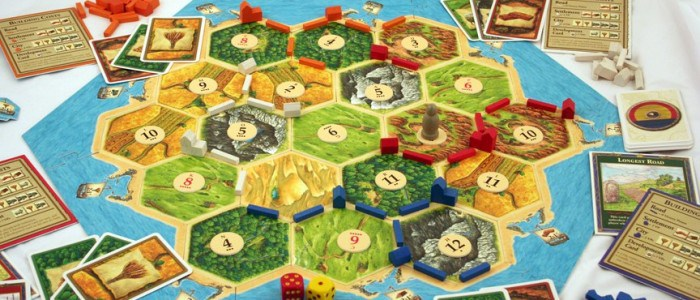
\includegraphics[width=\linewidth]{teaser.jpg}
}

%% Uncomment below to disable the manuscript note
%\renewcommand{\manuscriptnotetxt}{}

%% Copyright space is enabled by default as required by guidelines.
%% It is disabled by the 'review' option or via the following command:
% \nocopyrightspace

\vgtcinsertpkg

%%%%%%%%%%%%%%%%%%%%%%%%%%%%%%%%%%%%%%%%%%%%%%%%%%%%%%%%%%%%%%%%
%%%%%%%%%%%%%%%%%%%%%% START OF THE PAPER %%%%%%%%%%%%%%%%%%%%%%
%%%%%%%%%%%%%%%%%%%%%%%%%%%%%%%%%%%%%%%%%%%%%%%%%%%%%%%%%%%%%%%%%

\begin{document}

%% The ``\maketitle'' command must be the first command after the
%% ``\begin{document}'' command. It prepares and prints the title block.

%% the only exception to this rule is the \firstsection command
\firstsection{Introduction}

\maketitle

We have decided to work with the boardgame Settlers of Catan. The idea is to
visualize the effects of starting choices on the outcome of the game. It is a
game about managing odds and hedging your bets, so frequent players will be
interested in knowing what types of starting locations that gives a high
probability of winning.

\subsection{About the game}

Settlers of Catan is a game where you and a number of other players settle
an island. During the course of the game you acquire resources, build
improvements and acquire points. The first to 10 points wins the game.

For our project it is important to know that a settlement is located next
to 3 resource tiles with a number tile on top. Whenever the dice outcome is
the same as a number of a tile all players next to it receive a resource
token. Settlements can also be located next to the sea where there are harbors
that can be used to trade resources.

\section{Related work}

There have not been much work done on the topic, we have not been able to
find actual visualizations of the game, but we did find one analysis by Peter
Keep\cite{peter}. He attempts to use probabilities to estimate the worth of
resources and getting a gist of an optimal strategy. He never refers to his
dataset, but merely states things as known. He makes a good argument for his
approach to find the value of resources, but in his conclusions he fails to
take rarity of resources fully into account.

\section{Data and Task Abstractions}

\subsection{Domain Situation}

The target audience of the project is intermediate Settlers of Catan
players, who wants to get better at the game by getting a deeper understanding
of how to place the two starting settlements in order to maximize the chance
to win.

Relevant questions these players might ask would either be very concrete
in-the-moment questions or generally browsing for good combinations and things
to avoid. We imagine most players would be interested in just browsing the
data as well.

\begin{itemize}
  \item "What is the optimal settlement location?"
  \item "Is it feasible to settle without access to all resources?"
  \item "Does settling next to a desert always cause a loss?"
  \item "If my first settlement has wood and ore what resource should I go
    for?"
\end{itemize}

\subsection{Data and Task Abstractions}


The dataset\cite{lumin} consists of data for 50 4-player games. Each game
has 4 lines that consist of starting position, points gained, placements of
starting towns, total resource gains and losses from production, robber cards
and trade.

A snapshot of the dataset can be seen in appendix 1. We have mostly
used the data from the settlements and the points. The types of the attributes
can be seen in table \ref{tab:types}. It is worth nothing that the dices on
the resources are categorical because comparisons of them in this context is
meaningless.

\begin{figure}
  \centering
  \begin{tabular}{|l|l|}
    \hline
    Data & Type \\ \hline
    GameNum & Ratio \\ \hline
    Player & Categorical \\ \hline
    Points & Ratio \\ \hline
    Me & Categorical \\ \hline
    Dice throws & Categorical \\ \hline
    Settlement:res & Categorical \\ \hline
    Settlement:dice & Categorical \\ \hline
    Gains & Ratio\\ \hline
    Losses & Ratio \\ \hline
  \end{tabular}
  \caption{Attribute types}
  \label{tab:types}
\end{figure}

To win a game of Settlers you need 10 points and there will never be two
players with 10 or more points at the same time. However it is possible to
finish the game with 11 or 12 points, but this skews the data without being
particularly interesting when determining a winner, so we changed all values
above 10 to just 10.

Generally points are the main indicator of success in the game, so whenever we
need to analyze the quality of combinations we will measure it against points
and occasionally win-rate.

We did not consider gains and losses all that interesting. They are mostly
based on chance that is dependent on your settlements. We could show them, but
it would merely be a correlation between high gains and winning. The
experience Settler player would not be particularly interested in seeing this.

\section{Design}

Based on our data and task abstractions it would seem that the most important
part is the ability to view probabilities and to search the data for exact
situations. There are too many possible combinations for pie charts and the
probabilities do not relate to each other, so we stuck with simple bar
charts for the main part of our visualization.

What was more important was the filtering of data and we want to ensure that
any scenario can be created. We imagined doing this just with checkboxes, but
we modified this for implementation. We planned to make two rather basic
graphs and expand on them later.
\begin{figure}[!ht]
  \centering
  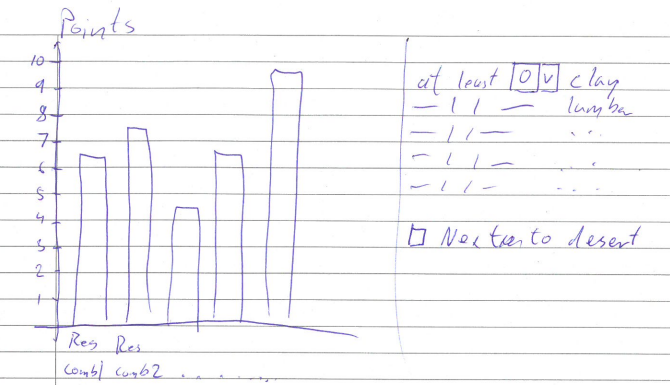
\includegraphics[width=\linewidth]{sketch1.png}
  \caption{Sketch of first graph}
  \label{fig:sketch1}
\end{figure}
In figure \ref{fig:sketch1} our first graph can be seen. It is a simple bar
chart with resource combinations matched to an average point score. There is a
checkbox and some dropdown menus to filter the results.
\noindent
\begin{figure}[!ht]
  \centering
  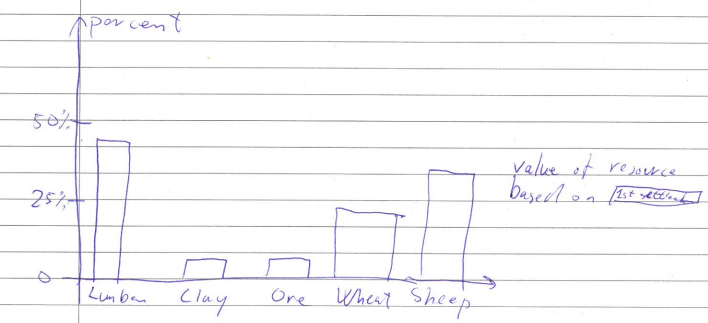
\includegraphics[width=\linewidth]{sketch2.png}
  \caption{Sketch of second graph}
  \label{fig:sketch2}
\end{figure}
\noindent
In figure \ref{fig:sketch2} the second graph can be seen. It shows the value
of resources based on points gained from games where the resources were
included. It can filtered to only show results based on one of the
settlements. 

\section{Implementation}

We implemented the visualization using the D3-library version 3. To make
data processing easier, We used python to transform the settlement columns
from a list of a comma separated values seen at fig \ref{tab:data}. Into
four columns with settlement position in one value and rolls on the specific
settlement, for both first and second settlement. All data processing were
done using javascript.

In our approach to making the visualization, we started out making a simple non
interactive bar chart using D3 of the first bar chart where we compared starting position to avg amount of points gained.
The x axis shows which resources the starting settlements had available as a string of each resource starting letter,
so "OOL" is ore, ore and wood for that given starting position and the y axis is average amount of points for that starting position.

Afterwards the filters were added and the bar chart updating each time a change is made.
To make it easier to see what each bar represented, we added popout boxes when
hovering over the bar's to show relevant information, we used the D3 tip library\footnote{https://github.com/Caged/d3-tip}
to do this.

The last thing we changed was adding the layered bar charts,
in bar chart 1, it is difficult to read the x axis, to try and solve this we layered
the bars to visualize each resource of the starting position with colors,
the size of each layer is based on how many of each resource the starting position has,
with beach and desert both having same color since they offer no value. With this bar chart
the size of each layer has no value with the y axis. In the 2. bar chart the size of each
layer represents the individual value the dice roll of the resource.

Due to the nature of having to learn each time we added new elements to our visualization, the code base became more cluttered and harder for us to add new features as we went along. If we had more time we would have cleaned up our code to make it easier to work in.
\section{Scenarios of use}

\subsection{Scenario 1}

”If my first settlement has two lumber and one ore what resources should I go
for?”

A user is in the middle of a game and has placed his first settlement next to
two lumber tiles and one ore tile. He wants to know what he should look for
when placing his second settlement.
\begin{figure}[!ht]
  \centering
  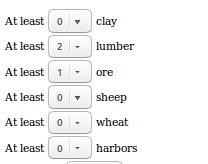
\includegraphics[scale=0.6]{scen1-1.png}
  \caption{Dropdown menu selection}
  \label{fig:s11}
\end{figure}
\noindent
He uses the drop downs menu and chooses settlements with at least 2 lumber
and 1 ore as seen in figure \ref{fig:s11}. The resulting graph is still rather
large, so he tries selecting "group duplicate resources" as seen in figure
\ref{fig:s12}.
\begin{figure}[!ht]
  \centering
  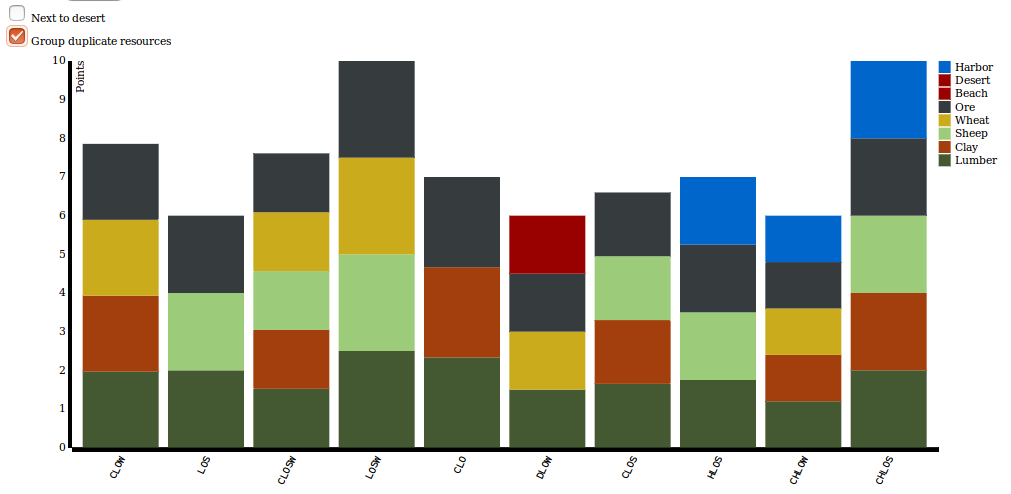
\includegraphics[width=\linewidth]{scen1-2.png}
  \caption{Grouped resources for the filter}
  \label{fig:s12}
\end{figure}
\noindent
From this he is able to gather that sheep and wheat
might just be the things to go for. Finally he scrolls to the second graph and
chooses to show "resource values based on second settlement" as seen in figure
\ref{fig:s13}.
\begin{figure}[!ht]
  \centering
  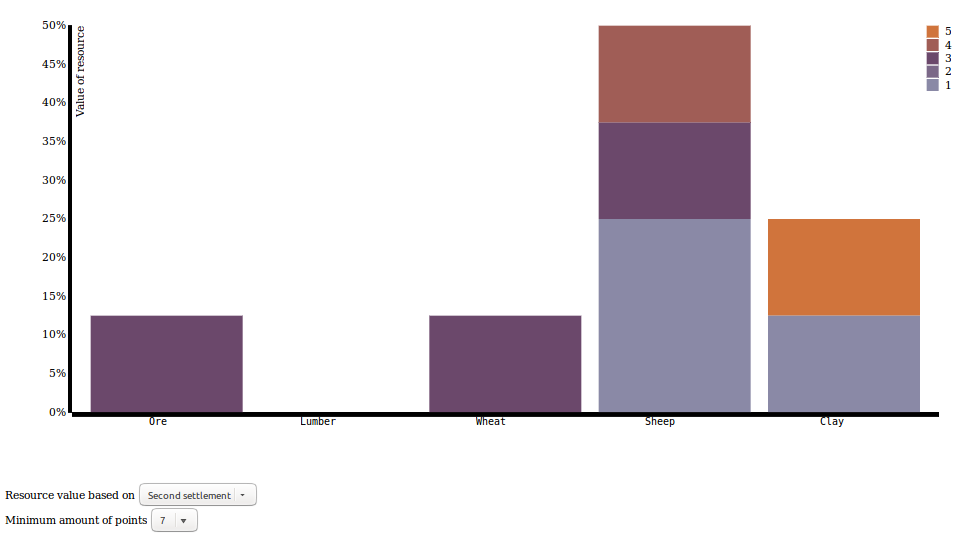
\includegraphics[width=\linewidth]{scen1-3.png}
  \caption{Value of resources for second settlement}
  \label{fig:s13}
\end{figure}
\noindent
Sheep has the highest value, but he only wants to compare to people who have
actually done well, so he sets minimum amount of points to 9 results can be
seen in figure \ref{fig:s14}. Sheep and Clay
look equally strong. He checks the dice values and decides that while he
can go for either or both, the dice value of the resource should be more
important than which one he chooses.
\begin{figure}[!ht]
  \centering
  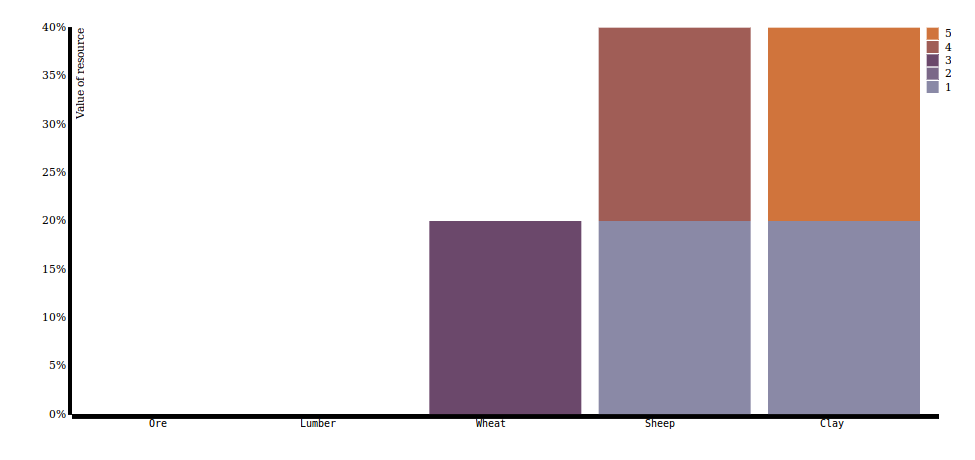
\includegraphics[width=\linewidth]{scen1-4.png}
  \caption{Resource values limited to players with at least 9 points}
  \label{fig:s14}
\end{figure}
\noindent

\subsection{Scenario 2}

"Should the desert be avoided at all cost?"

A user wants to know if it is feasible to place a city next to desert if the
other tiles are good. He ticks "next to desert" and sees 8 bars of data as
seen in figure \ref{fig:s21}. 
\begin{figure}[!ht]
  \centering
  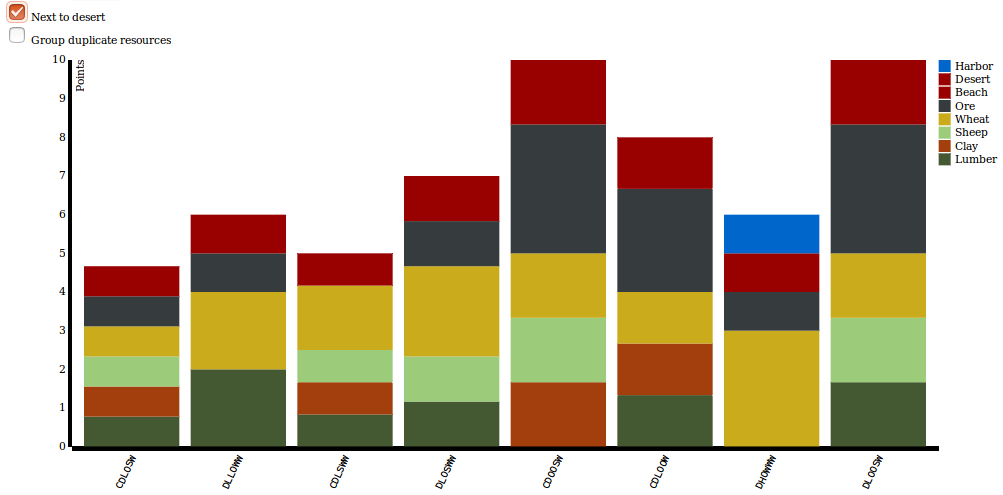
\includegraphics[width=\linewidth]{scen2-1.png}
  \caption{Limit to settlements next to desert}
  \label{fig:s21}
\end{figure}
\noindent
They are fairly spread, but he notices that some have won with it. He
scrolls to the second graph and sees that ore and wheat are the most valuable
resources in desert starts as seen in figure \ref{fig:s22}. 
\begin{figure}[!ht]
  \centering
  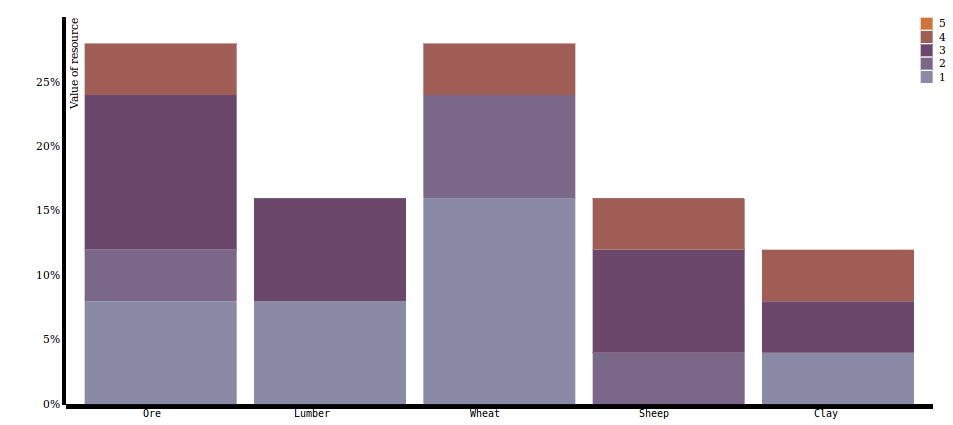
\includegraphics[width=\linewidth]{scen2-2.png}
  \caption{Second graph with desert}
  \label{fig:s22}
\end{figure}
\noindent
He tweaks the graph and the requires data to be
of players who have won the game as seen in figure \ref{fig:s23}. 
\begin{figure}[!ht]
  \centering
  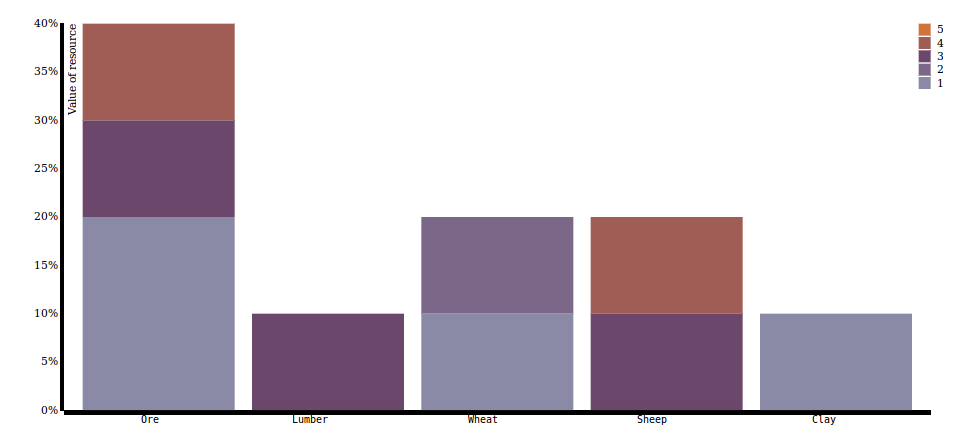
\includegraphics[width=\linewidth]{scen2-3.png}
  \caption{Limited to players with 10 points}
  \label{fig:s23}
\end{figure}
\noindent
He notices that as he increases the number
of required points wheat drops in value and ore remains the most important
resource. He also notices that your tiles needs to have good dices on them to
be valuable.

He concludes that good ore tiles can justify starting next to a desert.

\section{Discussion and Future Work}

Our visualization is not all we thought it would be. We had hoped that during
our implementation, through working with the data, we would come up with
more interesting visualization options, alas we are still using bar charts.
However the charts do a good job with data exploration, the filters are pretty
extensive and our second chart makes it pretty clear what you want to settle.
However, our project is a statistical project and simple bar charts do well
in this field. Another issue is that since implementation does some statistical
work, the results would have been more interesting if we instead of 200
data points had 20000. We have tried to make up for the lack of data, by
always writing the amount of data points, so the user will know to take it
with a grain of salt if there is just 1 case.

We would have liked to spend more time on the design step of the framework,
but everything got rushed so we had to prioritize getting started over getting
the design right. While aesthetics is not the priority of this course we would
have liked to make it all a little more pretty. The colors chosen for the
first graph are those used by the game itself with us adding color for
harbors, desert and beach. In the second graph we used a color scheme suited
for bars that relate somewhat to each other. 

We never came up with a better way to show the resource combinations on the
x-axis than their starting letters. We tried to do it with icons or colors,
but it just became a mess. Our choice to color the bars as well is messy,
particularly because the size of the segments means nothing, but it does make
the graph somewhat more readable. The initial graph is hard to read without
filters applied, but this was never the main intent of the it. We want the
user to filter down the data to something smaller, to explore the data by
creating scenarios.

All in all our implementation is not all we had hoped it would be, but we feel
it does a decent job at visualizing the data by doing the statistical work and
allowing the user to explore it.

%% if specified like this the section will be committed in review mode
\acknowledgments{
The authors wish to thank the Kaggle user "Lumin" for sharing his game stats}

%\bibliographystyle{abbrv}
\bibliographystyle{abbrv-doi}
%\bibliographystyle{abbrv-doi-narrow}
%\bibliographystyle{abbrv-doi-hyperref}
%\bibliographystyle{abbrv-doi-hyperref-narrow}

\bibliography{template}

\appendix
\newpage
\section{Appendix 1: Dataset}

Our dataset consists of 50 games each with 4 players. This makes for 200 lines
of data. In tabel \ref{tab:data} a condensed version of the data can be seen.
There are columns for all dice throws between 2 and 12.

\begin{figure}[h!]
  \centering
  \begin{tabular}{|l|l|l|l|l|l|l|l|l|l|l|l|}
    \hline
    GameNum & Player & Points & Me & 2 & ... & 12 & & & & & \\ \hline
    1 & 1 & 5 & & 1 & ... & 1 & & & & & \\ \hline
    1 & 2 & 9 & 1 & 1 & ... & 1 & & & & & \\ \hline
    1 & 3 & 10 & & 1 & ... & 1 & & & & & \\ \hline
    1 & 4 & 5 & & 1 & ... & 1 & & & & & \\ \hline \hline
    Set1 & & & & & & Set2 & & & & & \\ \hline
    6 & L & 3 & C & 11 & C & 9 & L & 10 & W & 11 & O \\ \hline
    5 & W & 8 & O & 10 & W & 4 & L & 5 & S & 11 & O \\ \hline
    5 & S & 6 & S & 12 & W & 8 & O & 4 & S & 3 & C \\ \hline
    6 & O & 9 & L & 3 & L & 4 & L & 8 & L & 10 & S \\ \hline \hline
    Production & TradeGain & RobberGain & TotalGain & TradeLoss & RobberLoss &
    Tribute & totalLoss & totalAvailable & & & \\ \hline
    38 & 5 & 2 & 45 & 10 & 2 & 4 & 16 & 29 & & & \\ \hline
    48 & 8 & 6 & 62 & 11 & 1 & 8 & 20 & 42 & & & \\ \hline
    44 & 14 & 9 & 67 & 24 & 4 & 0 & 28 & 39 & & & \\ \hline
    42 & 12 & 0 & 54 & 24 & 6 & 0 & 30 & 24 & & & \\ \hline
  \end{tabular}
  \caption{Dataset snapshot}
  \label{tab:data}
\end{figure}



\end{document}

